%
% LaTeX report template 
%
\documentclass[a4paper,11pt]{article}
\usepackage{graphicx}
\usepackage[english]{babel}
\usepackage{physics}
\usepackage{xcolor}
\usepackage{amsmath}
\usepackage{geometry}
\usepackage{titling}
\usepackage[hang, flushmargin, multiple]{footmisc}
\usepackage[unicode, colorlinks=true, linkcolor=blue, urlcolor=blue, citecolor=blue]{hyperref}
\usepackage{footnotebackref}

\graphicspath{ {images/} }

\setlength\parindent{0pt}

\geometry{
	left=1in,
	top=0.75in,
	bottom=0.75in,
	top=0.75in
}

%
\begin{document}
   \droptitle = -20mm
   \title{Notes on: FAQUAD in Quantum Dots}

   \author{David Fernandez Fernandez \\ e-mail: \href{mailto:david.fernandezf03@estudiante.uam.es}{david.fernandezf03@estudiante.uam.es}}
   
   \date{\today}

   \maketitle
   
   \tableofcontents
    

\section{Model}

The system that we study is a quantum dot (QD) array populated with heavy holes in presence of a external magnetic field perpendicular to the dots. Let us first consider the ideal case where there is no SO interaction and therefore the spin is conserved when hopping from one dot to the other. In this case the Hamiltonian is
\begin{equation}
H=\sum_{i\sigma}\varepsilon_{i\sigma}n_{i\sigma}+u\sum_in_{i\uparrow}n_{i\downarrow}-\sum_{i\neq j}\sum_\sigma\tau_{ij}\left(c_{i\sigma}^\dagger c_{j\sigma}+H.c.\right)\; ,
\label{eq:Hubbard_model}
\end{equation}
where $\varepsilon_{i\sigma}$ denoted the energy of the single-particle located in the dot $i$ with spin $\sigma=\uparrow,\downarrow=\pm1/2$. This energy takes into account the bias energy level of the dot and the Zeeman splitting
\begin{equation}
\varepsilon_{i\sigma}=\varepsilon_i+g\mu_B B\sigma\equiv \varepsilon_i+E_Z\sigma\; .
\end{equation}
A typical value of the effective $g$-factor for heavy holes in GaAs could be $g=1.35$. The intradot Coulomb interaction $u$ exist when various particles occupy the same dot. There is also a spin-conserving tunneling term $\tau$ between adjacent QD's. Finally, the operator $c_{i\sigma}$ ($c_{i\sigma}^{\dagger}$) represents the annihilation (creation) of a hole in the dot $i$ with spin $\sigma$.

\section{\label{sec:DQD}Double Quantum Dot}
The energy spectrum for a double quantum dot array (DQD) populated with two heavy holes is given in Fig.~\ref{fig:eigenenergies_2QD_2HH_wo_SOC}, where we have normalized the instant eigenenergies with the Zeeman splitting energy. It's usual to work with an antisymmetric bias gate for each dot where $\varepsilon_R=-\varepsilon_L$, and define the difference as the detuning $\varepsilon\equiv \varepsilon_R-\varepsilon_L$. To obtain this results we have excluded one of the double occupation states $\ket{S(2,0)}$, which is motivated by the setups where it's energy is much higher.
\begin{figure}[!htbp]
	\centering
	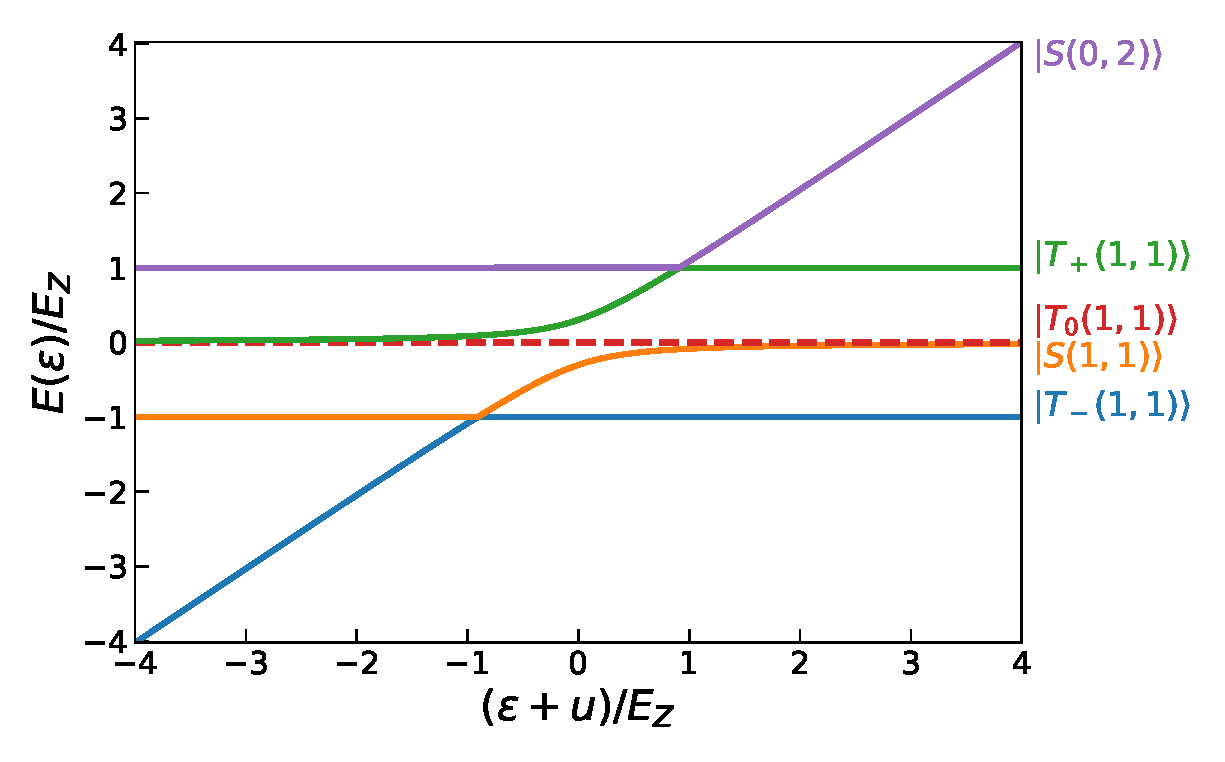
\includegraphics[width=0.8\linewidth]{eigenenergies_2QD_2HH_wo_SOC.eps}
	\caption{Energy spectrum for the system of a double quantum dot array populated with two heavy holes without spin orbit coupling. The parameters used are $B=0.015$~T, $E_Z=1.17\; \mu$eV, $\tau=0.25\; \mu$eV and $u=2$ meV.}
	\label{fig:eigenenergies_2QD_2HH_wo_SOC}
\end{figure}

We are only interested in the subspace formed by the two singlets states $\ket{S(1,1)}$, $\ket{S(0,2)}$, and the least energetic triplet estate $\ket{T_-(1,1)}$. With this the Hamiltonian can be easily written with the matrix
\begin{equation}
	H=\bordermatrix{~ & \ket{T_-(1,1)} & \ket{S(1,1)} & \ket{S(0,2)}\cr
		~ & -E_Z & 0 & 0 \cr
		~ & 0 & 0 & \sqrt{2}\tau \cr
		~ & 0 & \sqrt{2}\tau & \varepsilon+u \cr}\; .
\end{equation}
In order to couple the singlets and the triplet we can introduce two new terms, the Dresselhaus SOC and the Rashba SOC
\begin{equation}
	\begin{split}
	H_D&=\beta(\sigma_+p_-m_+p_--\sigma_-p_+p_-p_+)\\
	H_R&=i\alpha E_\perp (\sigma_+p_-^3-\sigma_+p_-^3)\; .
	\end{split}
\end{equation}
The ladder operators are defined by
\begin{equation}
	\begin{split}
	p_+\equiv p_x+ip_y\;, \quad p_-\equiv p_x-ip_y\;, 
	\end{split}
\end{equation}
where the momentum $p_x=-i\hbar \partial/\partial x$ and similar for $p_y$. To keep the computations as simpler as possible we take both SOC parameters to be equal $\beta=\alpha E_\perp$. The two new coupling terms are defined as
\begin{equation}
	\begin{split}
	\lambda_1&=\bra{T_-(1,1)}H_D+H_S\ket{S(1,1)}\\
	\lambda_2&=\bra{T_-(1,1)}H_D+H_S\ket{S(0,2)}\; .
	\end{split}
\end{equation}
To obtain an analytical expression for this two terms we can impose the single hole orbital functions with Gaussian shapes centered at each dot
\begin{equation}
	\psi_i=\frac{1}{l}\sqrt{\frac{2}{\pi}}\exp(-\frac{(x-x_i)^2+y^2}{l^2})\; ,
\end{equation} 
where the dot lies in the $x$ axis, $d$ is the interdot distance $x_1=-x_2=d/2$, and $l$ is the extent of the wave function. After integration we obtain the expressions
\begin{equation}
	\begin{split}
	\lambda_1&=\frac{8\alpha E_\perp d}{l^4}\exp(-d^2/l^2)\\
	\lambda_2&=\frac{4\sqrt{2}\alpha E_\perp d}{l^4}\exp(-d^2/2l^2)\; .
	\end{split}
\end{equation}
Choosing $l=d/3$ we observe that $\lambda_1/\lambda_2\approx 1/100$, being the coupling with the double occupation singlet states stronger. An analytical solution for the instant eigenstates is too complex, but we can solve it numerically, obtaining the energy spectrum shown in Fig~\ref{fig:eigenenergies_2QD_2HH_w_SOC}.
\begin{figure}[!htbp]
	\centering
	\includegraphics[width=0.8\linewidth]{eigenenergies_2QD_2HH_w_SOC.eps}
	\caption{Three lowest energies for the system of a double quantum dot array populated with two heavy holes in presence spin orbit coupling. The parameters used are $B=0.015$~T, $E_Z=1.17\; \mu$eV, $\tau=0.25\; \mu$eV, $\lambda_1=0.001\; \mu$eV, $\lambda_2=0.1\; \mu$eV and $u=2$ meV.}
	\label{fig:eigenenergies_2QD_2HH_w_SOC}
\end{figure}
Our task is to pass from $\ket{T_-(1,1)}$ to $\ket{S(1,1)}$ with the minimum possible occupation of $S(0,2)$. The reason is that we want to reduce as much as possible the charge noise produced when a hole ``jump" from one dot to another. We have not include any term in the Hamiltonian that flips the spin of the hole without ``jumping" to some other qubit, so the only possible transition allowed is
\begin{equation}
	\ket{\downarrow,\downarrow}\rightarrow \ket{0,\uparrow\downarrow} \rightarrow \frac{1}{\sqrt{2}}\left(\ket{\uparrow,\downarrow}-\ket{\downarrow,\uparrow}\right)\; .
\end{equation}
There exist some quasi adiabatic techniques that take advantage of the existence of a dark-state which has no weight in the intermediate step. To check if this is also the case for our system we can compute numerically the instant eigenvectors and extract the probability of the double occupation singlet state Fig~\ref{fig:occupation_middle_state}. Here we have plotted the value $|\braket{\psi_2}{S(0,2)}|^2$ where $\ket{\psi_2}$ correspond to the instant eigenstate in which we are interested (orange line in Fig~\ref{fig:eigenenergies_2QD_2HH_w_SOC}). To study the dependency with the tunneling we have assumed that both the spin-flip and spin-conserving rates are proportional to each other $\lambda_i\propto \tau$, specifically we have used $\lambda_2=0.25\tau$ and $\lambda_1=\lambda_2/100$. If we want to make a transition between the lowest energy triplet and the single occupation singlet we must go from $(\varepsilon(t_0)+u)/E_Z<-4$ to $(\varepsilon(t_f)+u)/E_Z>4$, this means that there is no dark state that does not populate $\ket{S(0,2)}$ in the range of detuning, unless the tunneling parameters are high enough.
\begin{figure}[!htbp]
	\centering
	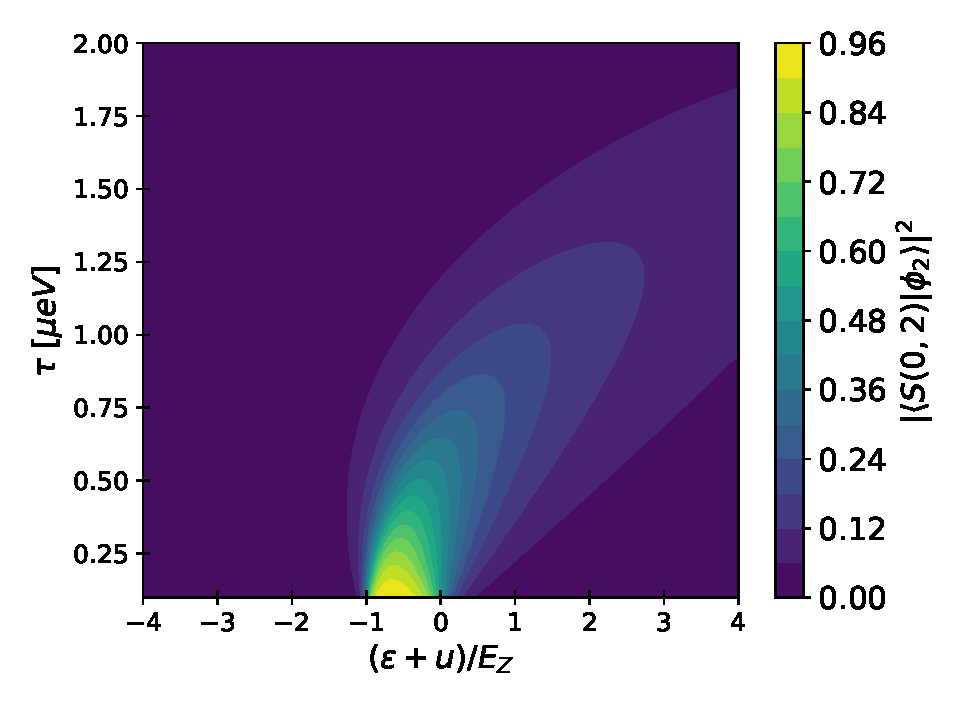
\includegraphics[width=0.6\linewidth]{occupation_middle_state.eps}
	\caption{Contribution of the double occupation singlet state in the instant eigenstate $\ket{\psi_2}$ in terms of the detuning and the spin conserving tunneling parameter $\tau$. For the SOC parameters we have set $\lambda_1=\lambda_2/100$ and $\lambda_2=0.25\tau$.}
	\label{fig:occupation_middle_state}
\end{figure}
The ideal situation is that at the beginning (end) of the protocol the instant eigenstate corresponds to $\ket{\phi_2(0)}=\ket{T_-(1,1)}$ ($\ket{\phi_2(t_f)}=\ket{S(1,1)}$). But this is only achieved with $\varepsilon\rightarrow -\infty$ ($\varepsilon\rightarrow \infty$), so we must decide the initial and final conditions for the protocol. The higher the limits for the detuning, the more adiabatic the transfer is, obtaining higher fidelities. The price to pay is higher energy consumption and longer total times. In Fig.~\ref{fig:limits_FAQUAD} we have plotted the population of the triplet and single occupation singlet states in $\ket{\phi_2}$ for different values of the detuning and the tunneling parameter. To maintain a balance between high fidelities and not very high detuning ranges, we will work with the limits given by $99.9\%$ of population. 
\begin{figure}[!htbp]
	\centering
	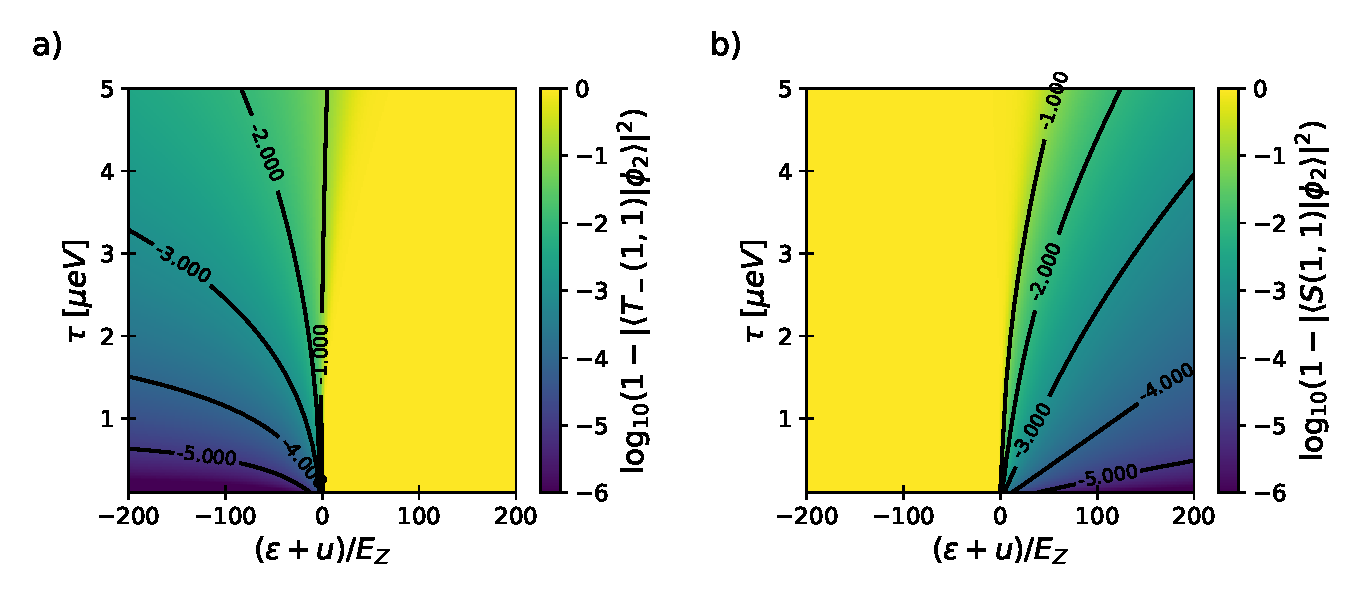
\includegraphics[width=\linewidth]{limits_FAQUAD.eps}
	\caption{Population of the states a) $\ket{T_-(1,1)}$ and b) $\ket{S(1,1)}$ in the instant eigenstate $\ket{\phi_2}$ in terms of the detuning and the tunneling. For the SOC parameters we have set $\lambda_1=\lambda_2/100$ and $\lambda_2=0.25\tau$.}
	\label{fig:limits_FAQUAD}
\end{figure}

\newpage
\section{FAQUAD}
The standard adiabaticity parameter is imposed to be constant, as
\begin{equation}
	\hbar\abs{\frac{\braket{\phi_1(t)}{\partial_t\phi_2(t)}}{E_1(t)-E_2(t)}}=c\; .
	\label{eq:adiabatic_parameter}
\end{equation}
To simplify the numerator we can use the definition of the instantaneous eigenstate for $\ket{\phi_2}$, derivate it with respect to time and multiply both side of the equation by $\bra{\phi_1}$, obtaining
\begin{equation}
	\begin{split}
	H\ket{\phi_2}&=E_2\ket{\phi_2}\\
	\bra{\phi_1}[(\partial_t H)\ket{\phi_2}+H\ket{\partial_t\phi_2}]&=\bra{\phi_1}[(\partial_t E_2)\ket{\phi_2}+E_2\ket{\partial_t\phi_2}]\\
	\bra{\phi_1}\partial_t H\ket{\phi_2}+E_1\braket{\phi_1}{\partial_t\phi_2}&=(\partial_t E_2)\braket{\phi_1}{\phi_2}+E_2\braket{\phi_1}{\partial_t\phi_2}\\
	\braket{\phi_1}{\partial_t\phi_2}&=\frac{\bra{\phi_1}\partial_t H\ket{\phi_2}}{E_2-E_1}\; ,
	\end{split}
\end{equation}
where in the third line we have used the orthogonality of the eigenstates $\braket{\phi_1}{\phi_2}=0$. With this we can rewrite the adiabaticity parameter in the form
\begin{equation}
\hbar\abs{\frac{\bra{\phi_1(t)}\partial_t H\ket{\phi_2(t)}}{[E_1(t)-E_2(t)]^2}}=c\; .
\end{equation}
This is only the case in which there are two states. If we consider a multilevel system the above equation is rewritten as
\begin{equation}
	\hbar \sum _{k\neq i}\abs{\frac{\bra{\phi_i(t)}\partial_t H\ket{\phi_k(t)}}{[E_i(t)-E_k(t)]^2}}=c\; ,
\end{equation}
where the index $i$ denotes the state in which we initialize the system. Using the chain rule we can write $\partial_t=\partial_\varepsilon \dot{\varepsilon}$ and the adiabatic condition is then
\begin{equation}
	\dot{\varepsilon}=\frac{c}{\hbar}\left(\sum _{k\neq i}\abs{\frac{\bra{\phi_i(t)}\partial_\varepsilon H\ket{\phi_k(t)}}{[E_i(t)-E_k(t)]^2}}\right)^{-1}\; .
	\label{eq:detuning_EDO}
\end{equation}
We can rescale the total operation time $t_f$ to $s\equiv t/t_f$ and define $\tilde{c}\equiv ct_f$, allowing us to write
\begin{equation}
	\tilde{c}=\int_{\varepsilon(0)}^{\varepsilon(t_f)}d\varepsilon\left(\sum _{k\neq i}\abs{\frac{\bra{\phi_i(t)}\partial_\varepsilon H\ket{\phi_k(t)}}{[E_i(t)-E_k(t)]^2}}\right)\; , 
	\label{eq:def_c_tilde}
\end{equation}
what can be easily computed numerically. If the condition $\tilde{c}/t_f\ll1$ is verified, them the transfer will remains adiabatic, and the wave function that describes the system can be expanded using adiabatic perturbation theory as
\begin{equation}
	\ket{\Psi(t)}=\sum_n a_n(t)e^{i\beta_n(t)}\ket{\phi_n(t)}
	\label{eq:adiabatic_wave_function}
\end{equation}
where we have defined the phase
\begin{equation}
	\beta_n(t)=-\frac{1}{\hbar}\int_0^tE_n(t')dt'+i\int_0^t\langle\phi_n(t')|\dot{\phi}_n(t')\rangle dt'\; .
\end{equation}
Introducing Eq.(\ref{eq:adiabatic_wave_function}) in the time dependent Schrödinger equation $i\hbar\partial_t\ket{\Psi(t)}=H(t)\ket{\Psi(t)}$ we can obtain a ODE for the amplitude of each instant eigenvector
\begin{equation}
	\begin{split}
	i\hbar\left[\sum_k \dot{a}_k(t)e^{i\beta_k(t)}\ket{\phi_k(t)}+ia_k(t)\dot{\beta}_k(t)e^{i\beta_k(t)}\right.&\ket{\phi_k(t)}+\\
	\left.+a_k(t)e^{i\beta_k(t)}|\dot{\phi}_k(t)\rangle\right] &= \sum_k g_k(t)e^{i\beta_k(t)}E_k\ket{\phi_n(t)}\\
	\sum_k\dot{a}_k(t)e^{i\beta_k(t)}\ket{\phi_k(t)}&=-\sum_k a_k(t)e^{i\beta_k(t)}|\dot{\phi}_k(t)\rangle.
	\end{split}
\end{equation}
Multiplying in both side by $\ket{\phi_n}$ with $n\neq k$ we obtain the equation
\begin{equation}
	\dot{a}_n(t)=-\sum_{k\neq n}a_n(t)e^{iW_{nk}(t)}\bra{\phi_n(t)}\dot{\phi}_k(t)\rangle\; ,
\end{equation}
where we have defined $W_{nk}(t)\equiv\int_0^t\omega_{nk}(t')dt'=\frac{1}{\hbar}\int_0^t[E_n(t')-E_k(t')]dt'$. Integrating the equation 
\begin{equation}
	a_n(t)-a_n(0)=-\sum_{k\neq n}\int_0^te^{iW_{nk}(t')}\bra{\phi_n(t')}\dot{\phi}_k(t')\rangle dt'\; .
\end{equation}
We the initial condition $\ket{\Psi(0)}=\ket{\phi_m}$ we can set as a first approximation $a_k(t)=\delta_{km}$. Using this in the above expression
\begin{equation}
	g_n^{(1)}(t)=-\int_0^te^{iW_{nm}(t')}\bra{\phi_n(t')}\dot{\phi}_m(t')\rangle dt'\; .
\end{equation}
As we can see in Eq.~(\ref{eq:adiabatic_parameter}), in a FAQUAD protocol we have $\bra{\phi_n(t)}\dot{\phi}_m(t)\rangle=cr\omega_{nm}(t)$, where we have defined the sign of the absolute value $r\equiv \operatorname{sgn}[\bra{\phi_n(t)}\dot{\phi}_m(t)\rangle\omega_{nm}]$. Using this in the above integral we have the final result
\begin{equation}
	g_n^{(1)}=-cr\int_0^t\omega_{nm}(t')e^{iW_{nm}(t')}dt'=icr\left(e^{iW_{nm}(t)}-1\right)\; .
\end{equation}
The population of the $n$-state is then given by the oscillatory function
\begin{equation}
	\abs{\braket{\phi_n(t)}{\Psi(t)}}^2=\abs{a_n(t)}^2=2c^2\left[1-\cos(W_{nm}(t))\right]\; .
	\label{eq:amplitude_undesired_states}
\end{equation}
The upper limit for the $n$-state population is $\abs{a_n(t)}^2\leq4c^2=4\tilde{c}^2/t_f^2$. In a two-level system the final population of the instant states have a period given by $T=2\pi/\Phi_{12}$ where the frequency is
\begin{equation}
	\Phi_{12}=\int_0 ^1 [E_1(s)-E_2(s)]ds\; .
\end{equation}

\subsection{FAQUAD in DQD: $\ket{T_-(1,1)}\rightarrow\ket{S(1,1)}$}
Let's apply the commented FAQUAD protocol to the system of two linear quantum dots populated with two heavy holes. The goal is to transfer the triplet state $\ket{T_-(1,1)}$ to the single occupation singlet $\ket{S(1,1)}$. The first step is to compute the adiabatic parameter $\tilde{c}$ solving numerically Eq.~(\ref{eq:def_c_tilde}). Setting $u=2$ meV, $E_Z=1.17\; \mu$eV ($B=15$ mT), $\tau=0.25 \; \mu$eV, $\lambda_2=0.1\; \mu$eV , $(\varepsilon(0)+u)/E_Z=-3$ and $(\varepsilon(t_f)+u)/E_Z=3$ we obtain a value of $\tilde{c}=4.31$ ns, so with typical times of $t_f\sim 10$ ns the adiabaticity parameter obtained is $c\sim 0.4< 1$ fulfilling the adiabatic condition. Once we have obtained the value for this parameter, which will remain constant during the hole transfer, we can numerically solve the ODE for the evolution of the detuning Eq.~(\ref{eq:detuning_EDO}). The result is shown in Fig.~\ref{fig:FAQUAD_detuning_2QD_2HH}, the dependency of this parameter with $s=t/t_f$ is plotted in a), while the derivative is represented in b) in terms of the detuning itself. We observe that when we reach the two avoided crossings the rate of change in the detuning decreases significantly, allowing an adiabatic passage, while in the rest of the point the velocity increases in order to speed up the transfer process.
\begin{figure}[!htbp]
	\centering
	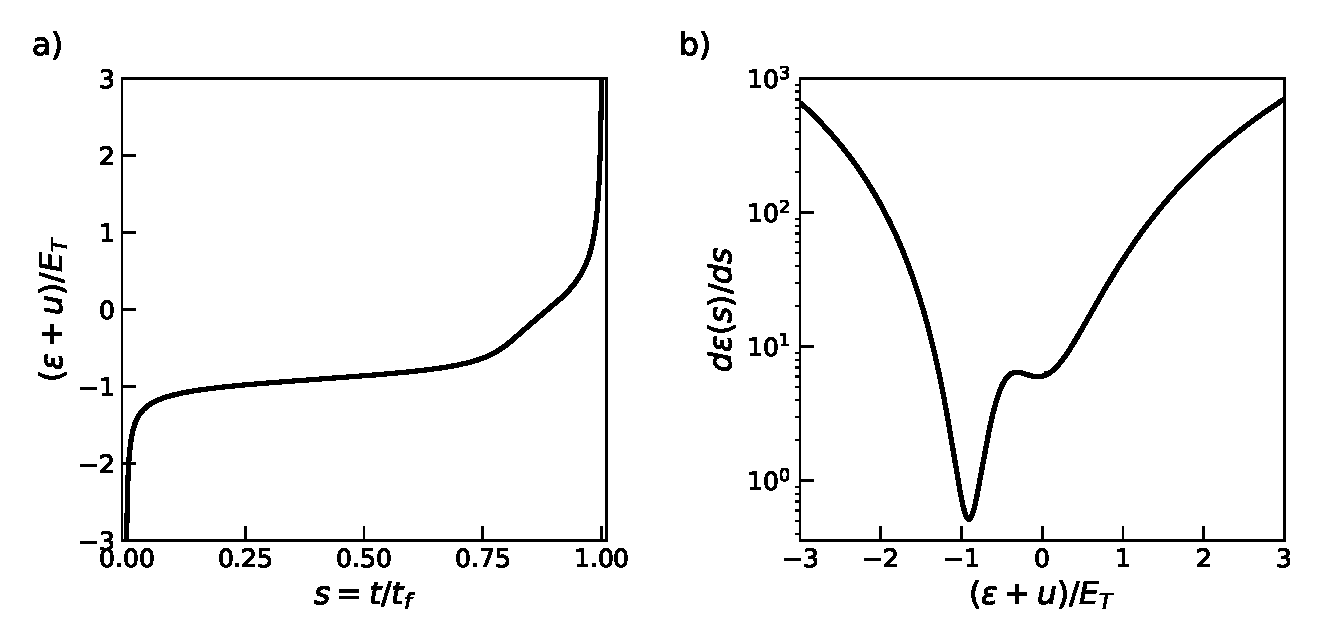
\includegraphics[width=1\linewidth]{FAQUAD_detuning_2QD_2HH.eps}
	\caption{Result obtained for the detuning after applying the FAQUAD protocol to the system of DQD populated with two HH. In a) the dependence of the detuning in terms of the adimensional parameters $s$. In b) the slope of the detuning $\varepsilon^\prime\equiv d \varepsilon/d s$ in terms of the detuning.}
	\label{fig:FAQUAD_detuning_2QD_2HH}
\end{figure}\\

We define the fidelity of this protocol as
\begin{equation}
	\mathcal{F}\equiv \abs{\braket{S(1,1)}{\Psi(t_f)}}^2\; .
\end{equation}
Computing this fidelity for different total times $t_f$ we obtain the results shown in Fig.~\ref{fig:FAQUAD_2QD_Results}. We can observe that the fidelity shows it's typical FAQUAD protocol behaviour, reaching a value close to the unit for large enough final times. In red we have plotted the lower bound for the fidelity, corresponding to the case in which $\ket{\phi_1}$ and $\ket{\phi_3}$ are populated with a probability given by $4\tilde{c}^2/t_f^2$. The first peak is reached at $t_f=18.17$ ns, with a fidelity of $\mathcal{F}=0.974$. In Fig.~\ref{fig:states_evolution} we have plotted the time evolution for the three different states for this value for the total operation time. We observe that the desired final state is obtained, but in the intermediate times the population of $S(0,2)$ is too high.
\begin{figure}[!htbp]
	\centering
	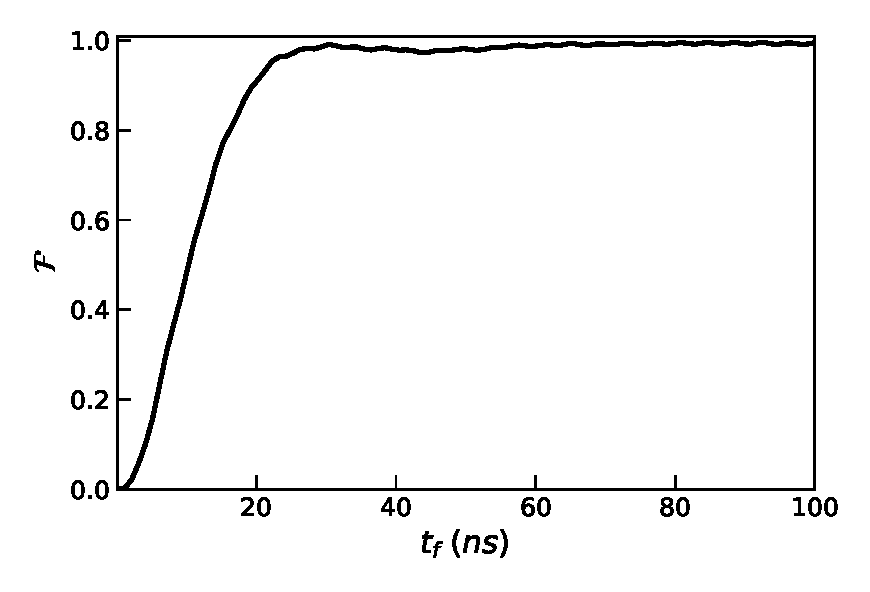
\includegraphics[width=0.7\linewidth]{FAQUAD_2QD_Results.eps}
	\caption{Result for the fidelity in terms of the total time of the protocol. The dashed red line represents the lower bound in which the two instant stares $\ket{\phi_1}$ and $\ket{\phi_3}$ are populated with probability $4\tilde{c}^2/t_f^2$. The tunneling parameter used is $\tau=0.25\; \mu$eV.}
	\label{fig:FAQUAD_2QD_Results}
\end{figure}

\begin{figure}[!htbp]
	\centering
	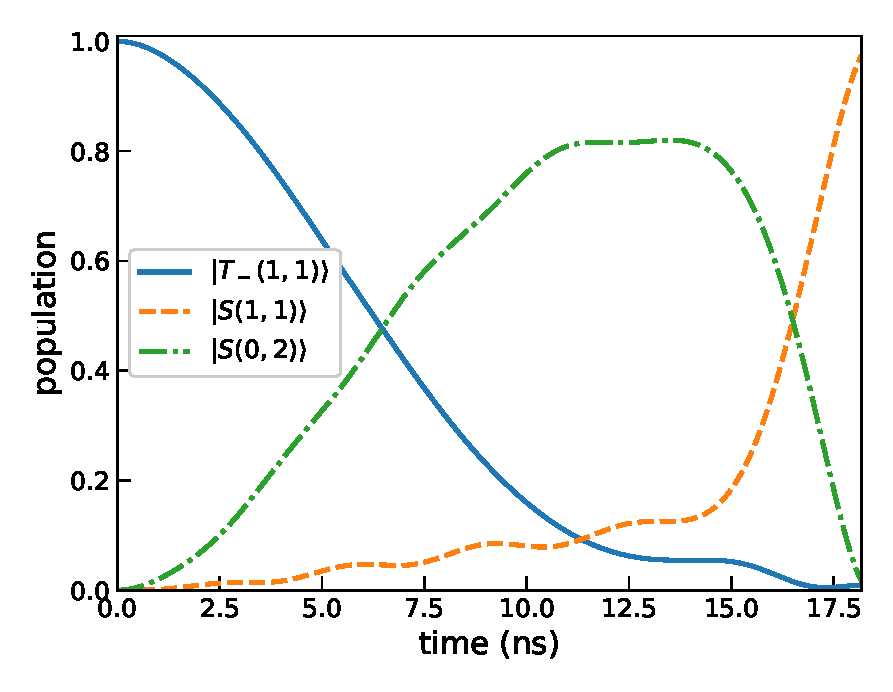
\includegraphics[width=0.7\linewidth]{states_evolution.eps}
	\caption{Evolution of the different states for the final time of $t_f=18.17$ ns and a fidelity $\mathcal{F}=0.974$. The tunneling parameter used is $\tau=0.25\; \mu$eV.}
	\label{fig:states_evolution}
\end{figure}

In order to decrease the population of $S(0,2)$ in the intermediate times we can increase the value of $\tau$. Setting the tunneling parameters $\tau=4 \; \mu$eV, $\lambda_2=1.6\;\mu$eV, and for the limits in the detuning $(\varepsilon(0)+u)/E_Z=-333$ and $(\varepsilon(t_f)+u)/E_Z=202$ we obtain an adiabatic parameter $\tilde{c}=1.17$ which is lower than before. This implies that the total times can be shorter in order to obtain the same fidelity. The fidelity in terms of the final time are shown in Fig.~\ref{fig:FAQUAD_2QD_Results_2}, with a first maximum of $\mathcal{F}=95.9\%$ at the time $t_f=4.67$ ns. As before let's plot the evolution of the system at this final time Fig.~\ref{fig:states_evolution_2}. We can see that the population of the double occupation singlet state $\ket{S(0,2)}$
\begin{figure}[!htbp]
	\centering
	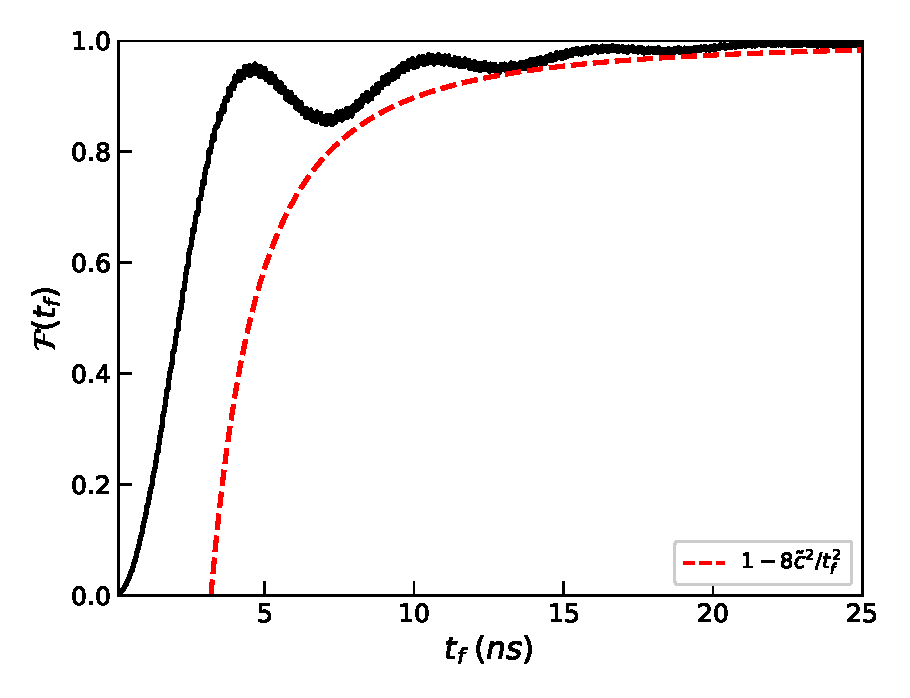
\includegraphics[width=0.7\linewidth]{FAQUAD_2QD_Results_2.eps}
	\caption{Result for the fidelity in terms of the total time of the protocol. The dashed red line represents the lower bound in which the two instant states $\ket{\phi_1}$ and $\ket{\phi_3}$ are populated with probability $4\tilde{c}^2/t_f^2$. The tunneling parameter used is $\tau=4\; \mu$eV.}
	\label{fig:FAQUAD_2QD_Results_2}
\end{figure}
\begin{figure}[!htbp]
	\centering
	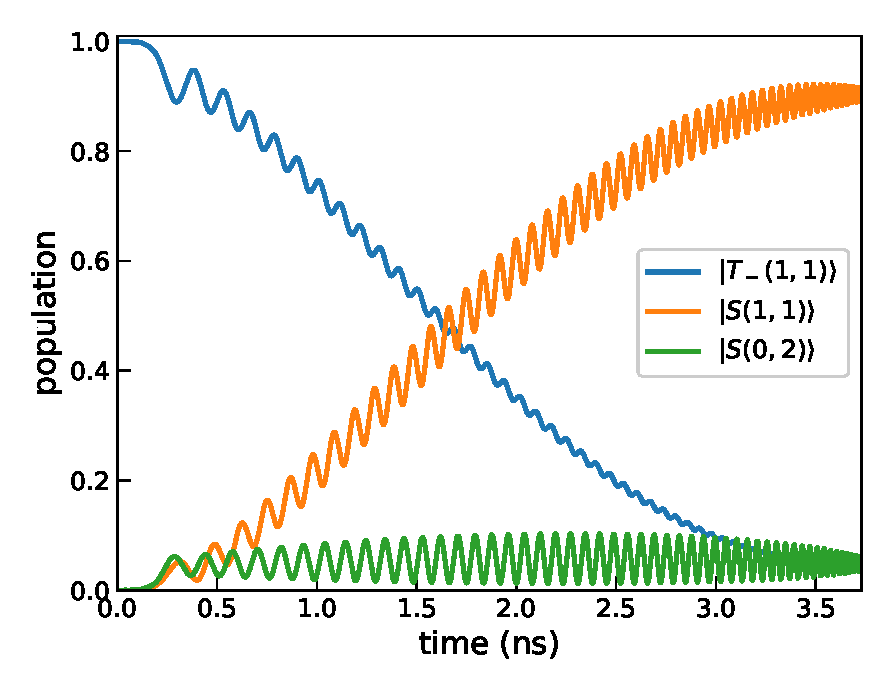
\includegraphics[width=0.7\linewidth]{states_evolution_2.eps}
	\caption{Evolution of the different states for the final time of $t_f=4.67$ ns and a fidelity $\mathcal{F}=0.96$. The tunneling parameter used is $\tau=4\; \mu$eV.}
	\label{fig:states_evolution_2}
\end{figure}\\

Recall that, at first order in adiabatic perturbation theory, the population of the states is given by Eq.~(\ref{eq:amplitude_undesired_states}). This means that the fidelity of the protocol can be described as
\begin{equation}
	\mathcal{F}^{(1)}(t_f)=1-4\tilde{c}^2/t_f^2[1-\cos(\Phi_{12}t_f)-\cos(\Phi_{23}t_f)]\; .
\end{equation}
Computing the values for the two characteristic frequencies $\nu_{nm}\equiv \Phi_{nm}/2\pi$ we obtain the values $\nu_{12}=1.41\; $ns$^{-1}$ and $\nu_{23}=9.11\; $ns$^{-1}$. In order to verify if the result obtained for the fidelity has this two frequencies we can compute the Fourier transform, obtaining the Fig.~\ref{fig:frecuency_spectrum}. With two red lines we have marked the predicted frequencies $\nu_{12}$ and $\nu_{23}$, which are present in the fidelity computed, but we can observe that there are two more important frequencies at $1.22\; \text{ns}^{-1}$ and $0.16\; \text{ns}^{-1}$.
\begin{figure}[!htbp]
	\centering
	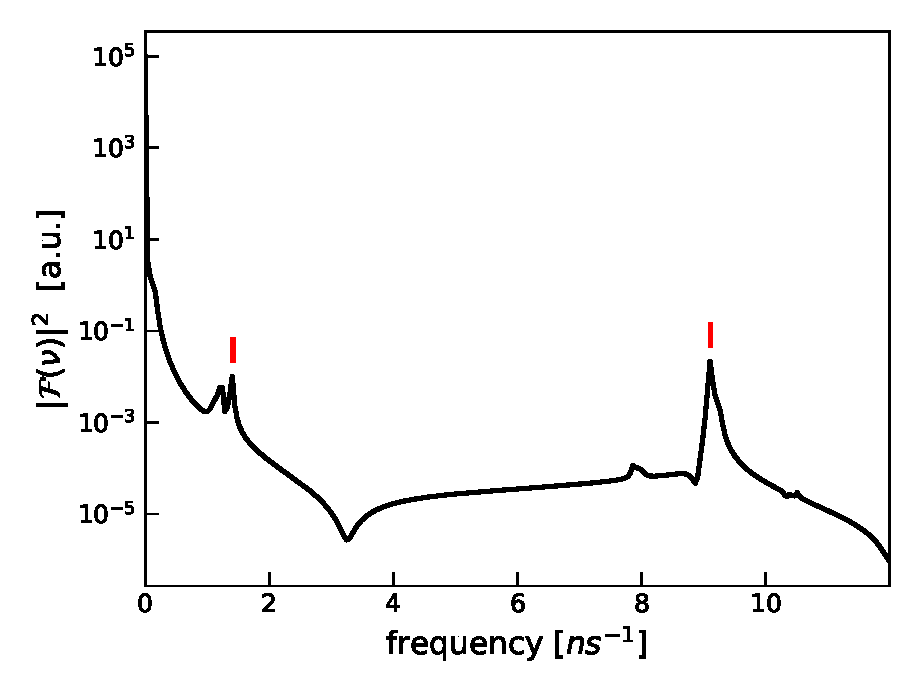
\includegraphics[width=0.7\linewidth]{frecuency_spectrum.eps}
	\caption{Fourier transform for the fidelity shown in Fig.~\ref{fig:FAQUAD_2QD_Results_2}. The two red lines are the predicted frequencies at first order in perturbation theory.}
	\label{fig:frecuency_spectrum}
\end{figure} 

We can check that increasing the value of $\tau$ and $\lambda_2$ has proved that the population $P_2(t)\equiv \abs{\braket{\Psi(t)}{S(0,2)}}$ has dropped  dramatically , in Fig.~\ref{fig:max_pop_S22} we plot the maximum population of this state in terms of the final time $t_f$. We have two possibilities to decrease even the population of the double occupation state, one of the is to increase even more the tunneling $\tau$. On the other hand we can use a slower transfer with higher values of $t_f$. The latter method is the least favourable because the population reaches a lower bound limit which depends on the particular value of $\tau$. I order to increase the fidelities obtained we have also to options, increase the total time as before or using a wider range for the detuning.
\begin{figure}[!htbp]
	\centering
	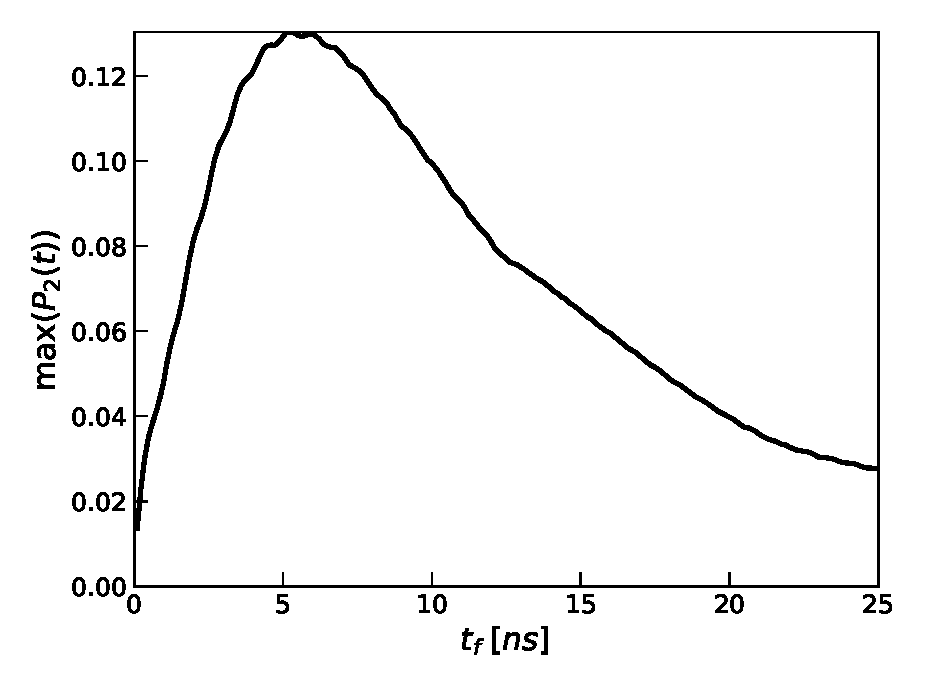
\includegraphics[width=0.7\linewidth]{max_pop_S22.eps}
	\caption{Maximum population of the state $S(0,2)$ for different values of the final time. The tunneling parameter used is $\tau=4\; \mu$eV.}
	\label{fig:max_pop_S22}
\end{figure}

\newpage
\appendix
\section{Equivalence between SOC Models}
In Sec.~\ref{sec:DQD} we have introduced the SOC with the terms
\begin{equation}
	\begin{split}
	\lambda_1&=\bra{T_-(1,1)}H_D+H_S\ket{S(1,1)}\\
	\lambda_2&=\bra{T_-(1,1)}H_D+H_S\ket{S(0,2)}\; ,
	\end{split}
\end{equation}
and the total Hamiltonian is then written as
\begin{equation}
H=\bordermatrix{~ & \ket{T_-(1,1)} & \ket{S(1,1)} & \ket{S(0,2)}\cr
	~ & -E_Z & \lambda_1 & \lambda_2 \cr
	~ & \lambda_1 & 0 & \sqrt{2}\tau \cr
	~ & \lambda_2 & \sqrt{2}\tau & \varepsilon+u \cr}\; .
\label{eq:Hamiltonian_Yue}
\end{equation}
Supposing Gaussian shapes for the wave functions, and with some given parameters we have obtained that $\lambda_1\ll\lambda_2$. In other references \cite{Bogan2018} the result is a little different. Using the Loewdin procedure we can redefine our basis orbitals as $\ket{\overline{L}}=\ket{L}-\frac{1}{2}S\ket{R}$ and $\ket{\overline{R}}=\ket{R}-\frac{1}{2}S\ket{L}$, where $S=\exp(-d^2/2l^2)$ is the overlapping of the original orbitals. Using this we obtain the expression for the spin flip tunneling
\begin{equation}
	\bra{\overline{L}\uparrow}H_D+H_S\ket{\overline{R}\downarrow}=-\alpha E_\perp \frac{d^3}{l^6}\exp(-\frac{d^2}{2l^2})-i\beta\left(\frac{4d}{l^4}-\frac{d^3}{l^6}\right)\exp(-\frac{d^2}{2l^2})\; .
\end{equation}
We will define this matrix element as $\bra{\overline{L}\uparrow}H_{\text{SOC}}\ket{\overline{R}\downarrow}\equiv -it_Fe^{i\delta}$, where the phase depends on the relative strength of the Rashba and Dresselhaus SOC. With this the Hamiltonian, in the atomic base, is written as
\begin{equation}
H_{\text{atomic}}=\bordermatrix{~ & \ket{\uparrow,\uparrow} & \ket{\uparrow,\downarrow} & \ket{\downarrow,\uparrow} & \ket{\downarrow,\downarrow} & \ket{0,\uparrow\downarrow}\cr
	~ & E_Z   			 & 0     & 0    & 0    			   & it_Fe^{-i\delta}  \cr
	~ & 0     			 & 0     & 0    & 0    			   & -\tau  		  	\cr
	~ & 0     			 & 0     & 0    & 0    			   & \tau 		  		\cr
	~ & 0     			 & 0     & 0    & -E_Z 			   & -it_Fe^{i\delta}   \cr
	~ & -it_Fe^{i\delta} & -\tau & \tau & it_Fe^{-i\delta} & \varepsilon+u}\; .
\end{equation}
Just by changing to the molecular base we obtain the matrix
\begin{equation}
H_{\text{molecular}}=\bordermatrix{~ & \ket{T_+(1,1)} & \ket{T_0(1,1)} & \ket{T_-(1,1)} & \ket{S(1,1)} & \ket{S(0,2)}\cr
	~ & E_Z   			 & 0     & 0      			  & 0    		   & it_Fe^{-i\delta}	 \cr
	~ & 0     			 & 0     & 0      			  & 0    		   & 0 		  	 		 \cr
	~ & 0     			 & 0     & -E_Z   			  & 0    		   & -it_Fe^{i\delta}    \cr
	~ & 0     			 & 0     & 0      			  & 0    		   & -\sqrt{2}\tau 		 \cr
	~ & -it_Fe^{i\delta} & 0     & it_Fe^{-i\delta}   & -\sqrt{2}\tau  & \varepsilon+u}\; .
\end{equation} We can restrict ourselves to the subspace $\ket{T_-(1,1)}, \ket{S(1,1)}, \ket{S(0,2)}$, computing the characteristic polynomial we have the equation
\begin{equation}
	(\varepsilon+u-x)x^2+x((\varepsilon+u-x)E_Z+t_F^2)+2(x+E_Z)\tau^2\; ,
\end{equation}
which does not depend on the exact phase of the spin flip tunneling, so we can set it to zero $\delta=0$. With this we can write the Hamiltonian for the sub-space in which we are interested as
\begin{equation}
H=\bordermatrix{~ & \ket{T_-(1,1)} & \ket{S(1,1)} & \ket{S(0,2)}\cr
	~ & -E_Z & 0 & -it_F \cr
	~ & 0 & 0 & \sqrt{2}\tau \cr
	~ & it_F & \sqrt{2}\tau & \varepsilon+u \cr}\; .
\end{equation}
This is indeed the same Hamiltonian that the one shown in Eq.~(\ref{eq:Hamiltonian_Yue}) under $\lambda_1\rightarrow 0$ and $\lambda_2\rightarrow -it_F$.

\newpage
\bibliographystyle{IEEEtran}
\bibliography{references}

\end{document}

